\documentclass[10pt,conference,compsoc]{IEEEtran}
\usepackage[utf8]{inputenc}
\usepackage{authblk}
\usepackage{graphicx}
\usepackage{url}
\usepackage{float}
\usepackage{amsmath}
\usepackage{algorithm}
\usepackage{algpseudocode}
\usepackage{multicol}
\usepackage{hyperref}
\usepackage{listings}
\usepackage{xcolor}

\hyphenation{}
\setcounter{secnumdepth}{4}
\setlength{\parindent}{0pt}
\setlength{\parskip}{0.5em plus 0.05em minus 0.15em}

% Stop LaTeX from stretching vertical glue to make columns flush; without this,
% leftover space is distributed between headings and paragraphs.
\raggedbottom

\lstdefinestyle{code}{
    basicstyle=\ttfamily\scriptsize,
    breaklines=true,
    frame=single,
    keywordstyle=\color{blue}\bfseries,
    columns=fullflexible,
    showstringspaces=false,
    captionpos=b,
    aboveskip=4pt,
    belowskip=6pt
}

\begin{document}

% Title and Author
\title{Techjam 2026: Task 3 Technical Report}
\author{Kevin Zhang}
\author{Isaac Ong}
\author{Hon Yi Hao}
\author{Danny Chan}
\affil{Group: Winner POV}
\date{31 August 2026}
\maketitle

% Abstract
\begin{abstract}
The disclosed test matrix for a fixed Transformer computation spans batch sizes, head dimensions and sequence lengths for which no single kernel performs best. We therefore submit a shape-aware dispatcher that selects among candidate kernel routes per input shape. Each route was first validated against the unmodified reference by comparing every output element against the stated tolerance, with any failing element disqualifying it, and only then timed using an interleaved measurement protocol. On an NVIDIA GeForce RTX 5080, the dispatcher passes 65/65 accuracy trials on test shapes 1--13 with zero failed elements, achieves a \textbf{3.611$\times$ geometric-mean speedup}, and reduces peak allocation by up to 90.4\%. It also makes test shape 14 executable in linear memory at 3.6\,GiB, where it passes five trials against a validated FP32 oracle.
\end{abstract}

% Introduction
\section{Introduction}
\IEEEPARstart{T}{he} task fixes the arithmetic of a Transformer layer and asks for GPU kernels that compute it faster while satisfying the executable per-element tolerance against a PyTorch reference. The reference, \texttt{torch\_transformer\_benchmark.py}, defines the model, inputs and checker; fourteen input shapes are disclosed in advance.

Table~\ref{tab:shapes} shows why the design works better when it selects implementations by shape check. We are able to categorize the disclosed test shapes into five different regimes:

\begin{enumerate}
    \item \textbf{Launch-bound} (Cases 2, 3, 4, 12). A forward pass finishes in about a millisecond, so kernel launch and Python dispatch dominate.
    \item \textbf{Memory-bound} (Cases 1, 5, 7, 9--11, 13). The $N \times N$ score tensor is read and written twelve times per layer to perform comparatively little matrix multiplication.
    \item \textbf{Projection-bound} (Case 8). At $d_\text{model}=1024$ and $N=128$ the dense GEMMs dominate and attention is only 15.7\% of the work.
    \item \textbf{Capacity-bound} (Case 6). A batch of 10{,}000 makes the dense activation set exceed 10\,GiB.
    \item \textbf{Allocation-bound} (Case 14). At $B{=}32$, $H{=}16$, $N{=}100{,}000$ the score tensor holds $5.12 \times 10^{12}$ values, or 20.48\,TB (18.63\,TiB) in FP32.
\end{enumerate}

As such, an optimization that wins in one regime may be neutral or harmful in another. For instance:

\begin{enumerate}
    \item \textbf{QKV projection fusion} (merging the Q/K/V projection matmuls into one GEMM):
    \begin{itemize}
        \item Case 3: $1.19\times$ speedup
        \item Case 8: $1.003\times$ speedup (no benefit)
    \end{itemize}
    \item \textbf{Degree-2 polynomial feature map}:
    \begin{itemize}
        \item Case 14: makes attention computation feasible
        \item Case 6: makes attention $186\times$ \emph{slower}
    \end{itemize}
    \item \textbf{FP16 internal execution behind an FP32 interface}:
    \begin{itemize}
        \item Two-layer Case 14: passes
        \item Four-layer shapes: fails
    \end{itemize}
\end{enumerate}

\begin{table}[H]
\centering
\scriptsize
\begin{tabular}{r r r r r r r l}
\hline
\textbf{\#} & \textbf{$B$} & \textbf{$d_\text{model}$} & \textbf{$H$} & \textbf{$N$} & \textbf{$L$} & \textbf{FFN} & \textbf{Class} \\
\hline
1  & 64     & 128  & 4  & 128     & 4 & 128  & memory-bound \\
2  & 1      & 128  & 4  & 128     & 4 & 128  & launch-bound \\
3  & 4      & 128  & 4  & 128     & 4 & 128  & launch-bound \\
4  & 16     & 128  & 4  & 128     & 4 & 128  & launch-bound \\
5  & 128    & 128  & 4  & 128     & 4 & 128  & memory-bound \\
6  & 10000  & 128  & 4  & 128     & 4 & 128  & capacity-bound \\
7  & 64     & 32   & 4  & 128     & 4 & 32   & memory-bound \\
8  & 64     & 1024 & 4  & 128     & 4 & 1024 & projection-bound \\
9  & 64     & 128  & 1  & 128     & 4 & 128  & memory-bound \\
10 & 64     & 128  & 2  & 128     & 4 & 128  & memory-bound \\
11 & 64     & 128  & 16 & 128     & 4 & 128  & memory-bound \\
12 & 64     & 128  & 4  & 32      & 4 & 128  & launch-bound \\
13 & 64     & 128  & 4  & 1024    & 4 & 128  & memory-bound \\
14 & 32     & 1024 & 16 & 100000  & 2 & 1024 & allocation-bound \\
\hline
\end{tabular}
\vspace{6pt}
\caption{The fourteen test shapes. Classification is derived from cost analysis as outlined in \S\ref{sec:method}.}
\label{tab:shapes}
\end{table}

From this analysis, we propose and submit a \emph{decision-based} kernel dispatcher. We report:

\begin{enumerate}
    \item A measurement methodology (\S\ref{sec:method}) for a machine whose clocks move 2$\times$ under sustained load, including a paired interleaved schedule and a per-run noise floor.
    \item A shape-aware dispatcher (\S\ref{sec:impl}) that routes on the disclosed tuple and runtime numerical contract.
    \item Final benchmark results on a GeForce RTX 5080 (\S\ref{sec:results}).
    \item An account of how AI assistance was used (\S\ref{sec:ai}).
\end{enumerate}

\section{Problem and Correctness}

\subsection{Reference Computation}
Each block applies pre-norm attention and a pre-norm GELU feed-forward network with residual additions, with the model applying a final LayerNorm. Here, attention is written in Listing~\ref{lst:ref}:
\vspace{0.5cm}

\begin{lstlisting}[style=code,caption={The reference attention core, abridged from \texttt{BaselineSelfAttention.forward}.},label={lst:ref}]
scores = torch.matmul(q, k.transpose(-2, -1)) * self.scale
causal_mask = torch.ones((N, N), dtype=torch.bool,
                         device=x.device).triu(diagonal=1)
scores = scores.masked_fill(causal_mask, float("-inf"))
scores = scores.masked_fill(invalid_keys, float("-inf"))
probs = torch.softmax(scores.float(), dim=-1).to(dtype=x.dtype)
output = torch.matmul(probs, v)
\end{lstlisting}

\subsection{Executable Criterion}
An output element passes when
\begin{equation}
\lvert c - r \rvert \le 0.002 \;\;\lor\;\; \lvert c - r \rvert \le 0.02\,\lvert r \rvert ,
\label{eq:tol}
\end{equation}
where $c$ is the candidate value and $r$ the reference value.

\subsection{Constraints}
The reference rounds attention probabilities back to the model dtype before multiplying by $V$. Under a float16 reference, this makes free rewrites unsafe, as folding the $1/\sqrt{d_k}$ scale into $Q$ flips both Cases 7 and 13 to fail. We therefore target float32 for the four-layer cases.

\section{Analysis and Benchmarking Methodology}
\label{sec:method}

\subsection{Analytic Cost Model}
Each shape family was first characterized in order to better focus our optimization strategies. For instance, for Case 13 ($B{=}64$, $H{=}4$, $N{=}1024$, $d_h{=}32$) the score tensor $S$ holds $2.68\times10^{8}$ elements, or 1.00\,GiB in FP32. Scaling, two masked fills and the three-pass softmax each read and write $S$. Relative to the GPU's compute-to-bandwidth balance, the resulting arithmetic intensity places attention firmly in the memory-bound regime.

However, for Case 14, attention is about 95\% of all FLOPs, roughly 0.655\,PFLOP per causal layer. Hence, FLOP reduction is the biggest factor that can speed-up computation.

\subsection{Operator-Level Attribution}
Analysis was confirmed with the PyTorch profiler with NVTX ranges at each stage. Figure~\ref{fig:attribution} shows the result for Case 13 eager attention, as the actual attention matmul is the smallest cost, while the layout copies produced by \texttt{.contiguous()} in \texttt{\_split\_heads} are 7.1$\times$ larger.

\begin{figure}[H]
\centering
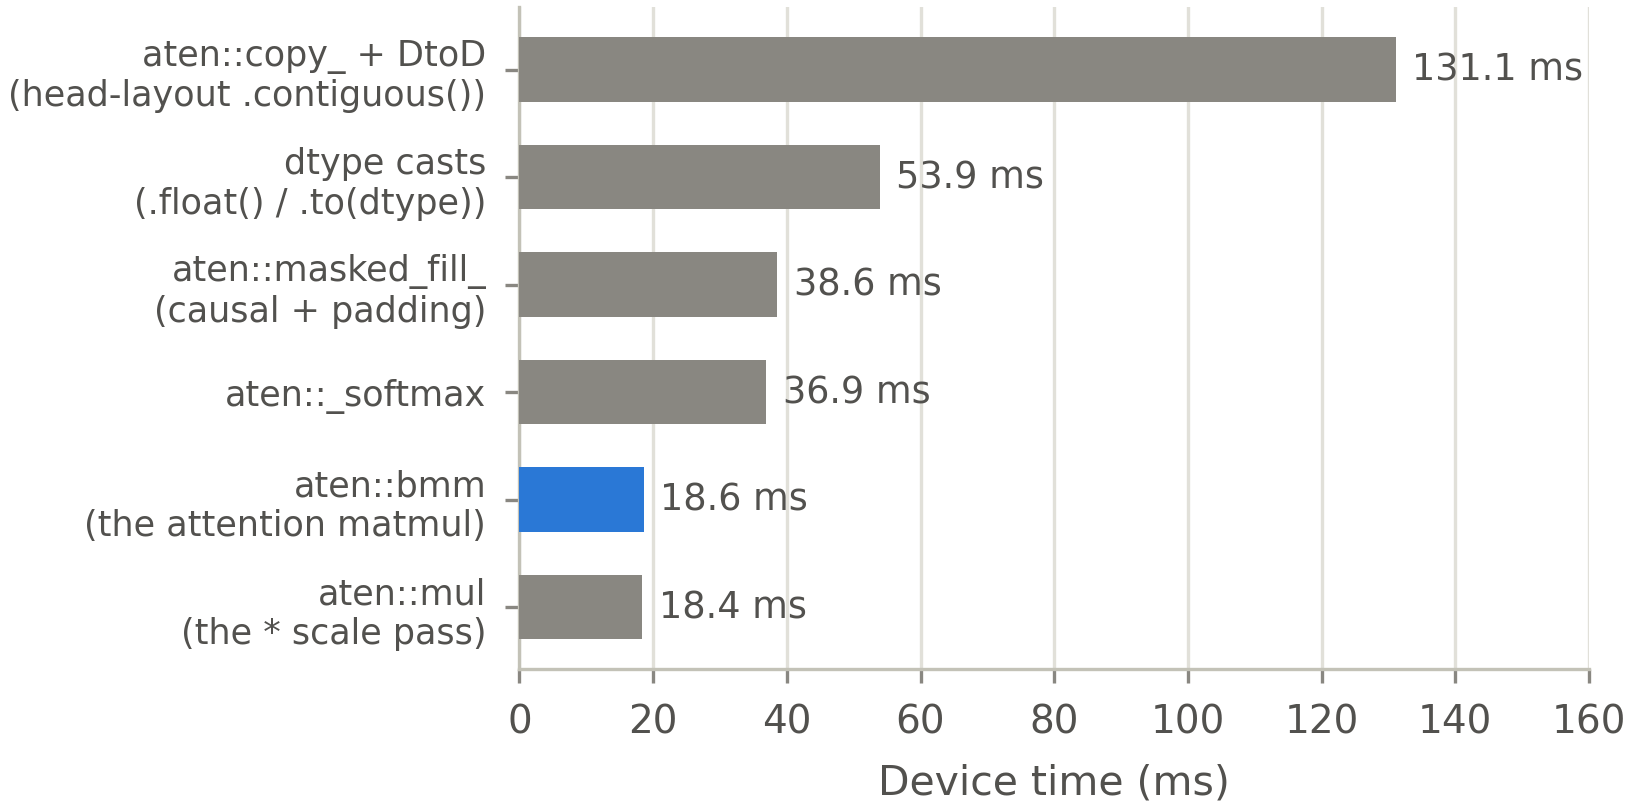
\includegraphics[width=\linewidth]{fig/attention-time-attribution.png}
\vspace{6pt}
\caption{Where Case 13's eager attention time actually goes, by operator. The operator that performs the attention arithmetic is highlighted.}
\label{fig:attribution}
\end{figure}

\subsection{A/B Timing Measurement}
\label{sec:timing}
Our development GPUs do not hold a stable clock, so a schedule that measures one implementation entirely before the other can report inconsistent speedups. Empirically, identical code drifted 17.5\% between sessions minutes apart, and four identical profiles spread 2.17$\times$.

Three mechanisms address this, which can be found in \texttt{src/infra/timing.py}.

\subsubsection{Settling}
Iteration-count warmup is insufficient because the boost budget is spent in wall-clock time. Hence, each arm is instead held under continuous load for a fixed 10 seconds.

\subsubsection{Interleaved paired schedule}
Samples are emitted as alternating \texttt{AB} and \texttt{BA} pairs, which gives both labels the same mean position in the run and cancels monotonic drift.

\subsubsection{Noise Floor from Within-Pair Disagreement}
Because baseline and candidate are timed back to back, each pair sees the same clock and thermal state, so their ratio $\rho_i = b_i / c_i$ is unaffected by drift across the run. Any remaining variation between pairs reflects the run's own measurement noise. We quantify this noise floor as the half-width of a 95\% confidence interval around the median of these ratios,
\begin{equation}
\phi \;=\; 1.96 \cdot \frac{1.2533 \cdot \operatorname{sd}(\rho)}{\sqrt{n}} ,
\label{eq:noise}
\end{equation}
where $1.2533$ converts the standard error of the mean to that of the median. A measured speedup $s$ is accepted only when $\lvert s - 1 \rvert > \phi$, i.e. only when it exceeds what the run's own noise could produce by chance. For launch-bound shapes, we batch several forward passes into each timed sample, sized automatically to target 50\,ms per block to average out scheduling noise.

\subsection{AI-Assisted Development}
\label{sec:ai}
AI agents (Codex GPT 5.6 and Claude Opus 5) were used to perform research, repository and upstream-source inspection, task decomposition, profiler-trace interpretation, hypothesis generation, implementation, cross-stream conflict review, benchmark orchestration and documentation.

We only treat an AI suggestion as a hypothesis, and all optimization changes were manually reviewed by each member before integrating it into the main branch. Here are some judgement calls we had to make in our implementation:

\begin{itemize}
    \item An agent recommendation to pack Q/K/V universally was narrowed to Cases 2 and 3 after the end-to-end screen on Case 8 measured 1.003$\times$.
    \item A blanket ``FP16 fails'' statement was found to be too general, as by testing, we found that it does not hold for FP16 internal compute behind an FP32 interface, which passes on Case 14.
    \item An attention-core speedup was correctly distinguished from a whole-model speedup after a microbenchmark and a full run disagreed by more than an order of magnitude.
    \item A numerical guard threshold initially proposed at 0.60, and later measured at 0.45, had to be lowered again to 0.40 after testing (\S\ref{sec:guard}).
\end{itemize}

\section{Implementation}
\label{sec:impl}
The submitted candidate is \texttt{DispatchingTransformer} in \texttt{src/dispatcher.py}. It subclasses the reference transformer, so it inherits the exact parameter names and the exact block structure, and replaces only the attention module and the forward entry point.

\subsection{Routing Key}
Routing is decided on the tuple \emph{and} the runtime numerical contract:
\begin{equation*}
(B,\, N,\, d_\text{model},\, H,\, \text{FFN},\, \text{causal},\, L)
\end{equation*}
identifies the official case, and a separate runtime key carries the input shape, device type and index, dtype, device name and compute capability, mask presence, inference/grad state, float32 matmul precision and the TF32 flag. Anything else falls back to the reference arithmetic.

Compilation is lazy and cached per model instance and runtime key, the cache is invalidated by anything that could change correctness, and any compiled call that raises at runtime demotes permanently to the reference path.

\subsection{Compiled Float32 SDPA}
Cases 1--5 and 7--12 replace score materialization with \texttt{scaled\_dot\_product\_attention} under \texttt{torch.compile(mode=\allowbreak'reduce-overhead')}; Cases 2 and 3 additionally use the packed-QKV route described below. Case 13 uses default compilation, which performed better for its larger compute- and memory-bound graph. This substitution delivers four of the levers identified in \S\ref{sec:method} at once:
\begin{enumerate}
    \item the score tensor is never materialized \cite{rabe,flash2};
    \item the softmax runs as a single online pass \cite{online};
    \item normalization is deferred to the $[B,H,N,d_h]$ output;
    \item causal block-skipping is already implemented inside the operator.
\end{enumerate}

Compiler mode was chosen via analysis and measurement. For instance, for launch-bound shapes like Case 2, \texttt{reduce-overhead} measured $6.581\times$ against only $2.212\times$ for default mode, since \texttt{reduce-overhead} is specifically designed to cut this per-call overhead via CUDA graphs.

\subsection{Layout and Mask Elimination}
SDPA accepts strided inputs, so \texttt{.contiguous()} copies in \texttt{\_split\_heads} are avoidable. Hence, replacing them with transposed views adds a further 6--12\% on top of SDPA and removes the largest item in Figure~\ref{fig:attribution}.

Additionally, we can remove the padding key mask for right-padded masks, as causal masking already writes $-\infty$ at every position the padding mask would, and the reference separately zeroes the invalid query rows. This condition is checked as a left-padded or interior-hole mask is not removable, so the dispatcher classifies the mask once per runtime key on the host and bakes the decision in before tracing.

\subsection{Case 2 \& 3: Packed QKV Projections}
Cases 2 and 3 combine the three projection GEMMs into one. Both are launch-bound shapes, where runtime is dominated by per-kernel launch and dispatch overhead rather than by the GEMMs' own compute time; collapsing three launches into one removes overhead directly in the regime where overhead is the bottleneck. The packed weight is rebuilt outside timed execution, refreshed by a \texttt{load\_state\_dict} post-hook, and preserves the reference parameter names so strict weight loading still succeeds.

\subsection{Case 6: Batch Streaming}
Case 6's difficulty is being capacity-bound because a batch of 10{,}000 does not fit in memory at once. We handle this by streaming the batch through a bounded float32 SDPA path in chunks. Chunk size is chosen as the largest power of two that fits a memory budget computed from live free memory, the reusable allocator cache, and a cap of 85\% of total VRAM. If an allocation still fails, the chunk size is halved and the attempt is retried.

\subsection{Case 14: Streaming, Mixed Precision and Guarded Linear Attention}
Case 14 is the only shape that cannot execute from the reference arithmetic, as its dense FP32 score tensor is 20.48\,TB (18.63\,TiB), and its input and output together occupy about 24.4\,GiB. Hence, the following sections elaborate on the three separate mechanisms that enable it to run.

\subsubsection{Prefix streaming}
The route processes one sample's valid prefix at a time and passes no attention mask. It therefore avoids retaining full-batch intermediate activations proportional to $B \cdot N \cdot d_\text{model}$, while the bounded working set for each streamed sample still scales with $N \cdot d_\text{model}$.

\subsubsection{FP32 interface, FP16 compute}
Parameters and the input/output interface remain FP32. Each streamed sample is cast to FP16 internally, and both Transformer blocks execute their attention, feed-forward and residual arithmetic in FP16 before the result is returned through the FP32-facing route.

\subsubsection{Polynomial feature-map attention}
At $N{=}100{,}000$ the path is compute-bound, so we focused on reducing FLOPs directly. We approximate $\exp(s)$ with the degree-2 polynomial that is $L^2$-optimal under the measured score distribution $s \sim \mathcal{N}(0,\sigma^2)$. The Gauss--Hermite projection gives
\begin{equation}
\exp(s) \;\approx\; e^{\sigma^{2}/2}\!\left[\left(1 - \tfrac{\sigma^{2}}{2}\right) + s + \tfrac{s^{2}}{2}\right],
\label{eq:poly}
\end{equation}
The $e^{\sigma^2/2}$ factor must be kept, since the block computed exactly along the diagonal uses unscaled $\exp$ and the two must remain on a consistent scale. Because Eq.~\ref{eq:poly} is a polynomial in $s = a \cdot b$, it can be rewritten as an explicit inner product. With $a = q\sqrt{\text{scale}}$ and $b = k\sqrt{\text{scale}}$, the feature map
\begin{equation*}
\phi(a) = \left[\sqrt{c_0},\; \sqrt{c_1}\,a,\; \sqrt{c_2}\,\mathrm{vec}(a a^{\top})\right]
\end{equation*}
satisfies $\phi(a)\!\cdot\!\phi(b) = c_0 + c_1(a\!\cdot\!b) + c_2 (a\!\cdot\!b)^2 \approx \exp(a \cdot b)$. Substituting this feature map turns causal attention into a chunked linear scan with a running state of size $O(d_f d_h)=O(d_h^3)$ and total work $O(N d_f d_h)=O(N d_h^3)$, rather than the $O(N^2 d_h)$ work of exact attention \cite{katharopoulos}. The construction is a deterministic relative of Performer's random features \cite{performer} and the second-order Taylor map of BASED \cite{based}.

The polynomial approximation is least accurate for early tokens, whose short causal prefixes provide fewer keys over which approximation errors can average out. We therefore compute the first 4{,}096 tokens exactly, which costs only 0.17\% of the full quadratic work but cuts maximum error from $6.6\times10^{-3}$ to $1.8\times10^{-3}$.

The polynomial route uses three fused Triton entry points---quadratic apply, quadratic update and the exact causal diagonal---that construct $a a^{\top}$ directly in registers \cite{triton}. This avoids materializing the $C \times d_h^2$ feature tiles in HBM and removes roughly 51\,GB of cumulative feature traffic per sample-layer at the Case 14 shape. The exact-prefix correction itself uses SDPA.

\subsubsection{Where Crossover Favours Linear Attention}
The method trades $O(N^2 d_h)$ for $O(N d_h^3)$, so it wins when
\begin{equation}
N \;>\; 2 d_h^{2}.
\label{eq:crossover}
\end{equation}
Figure~\ref{fig:crossover} places all fourteen shapes against the boundary of Eq.~\ref{eq:crossover}, and only Case 14 is on the profitable side.

\begin{figure}[H]
\centering
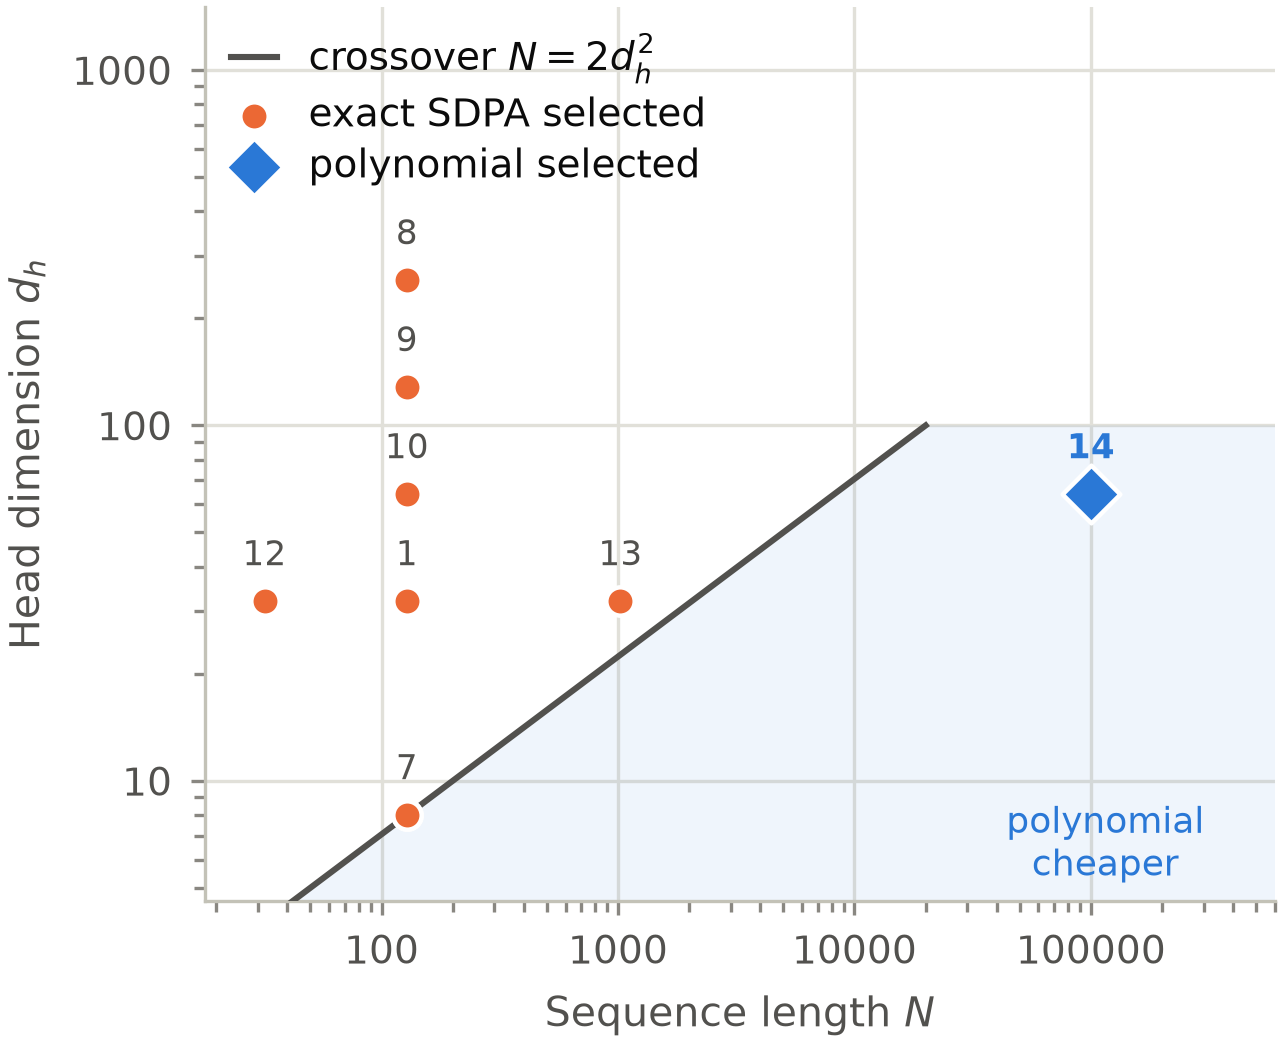
\includegraphics[width=\linewidth]{fig/poly-crossover.png}
\vspace{6pt}
\caption{Linear attention is cheaper than exact causal attention only above $N = 2d_h^2$. Only Case 14 sits far inside the shaded region.}
\label{fig:crossover}
\end{figure}

\subsubsection{The runtime guard}
\label{sec:guard}
The approximation's accuracy depends on $\sigma$, which is a property of the benchmark's random initialization. Under trained weights, scores are far larger and a degree-2 fit would be poor. To prevent this, the route is gated at runtime: $\sigma$ is estimated from a 512-row sample, and the polynomial path runs only when $\sigma \le 0.40$. Otherwise, the route forces exact Flash SDPA.

The ceiling was set by the sweep in Figure~\ref{fig:sigma}, obtained by scaling Q/K/V projection weights of both reference and candidate and recording where the criterion first fails. Additionally, the failure count is not monotonic near the boundary. Therefore, we placed $\sigma$ (0.40) below the largest clean pass at 0.4188 and 20\% above the operating point.

\begin{figure}[H]
\centering
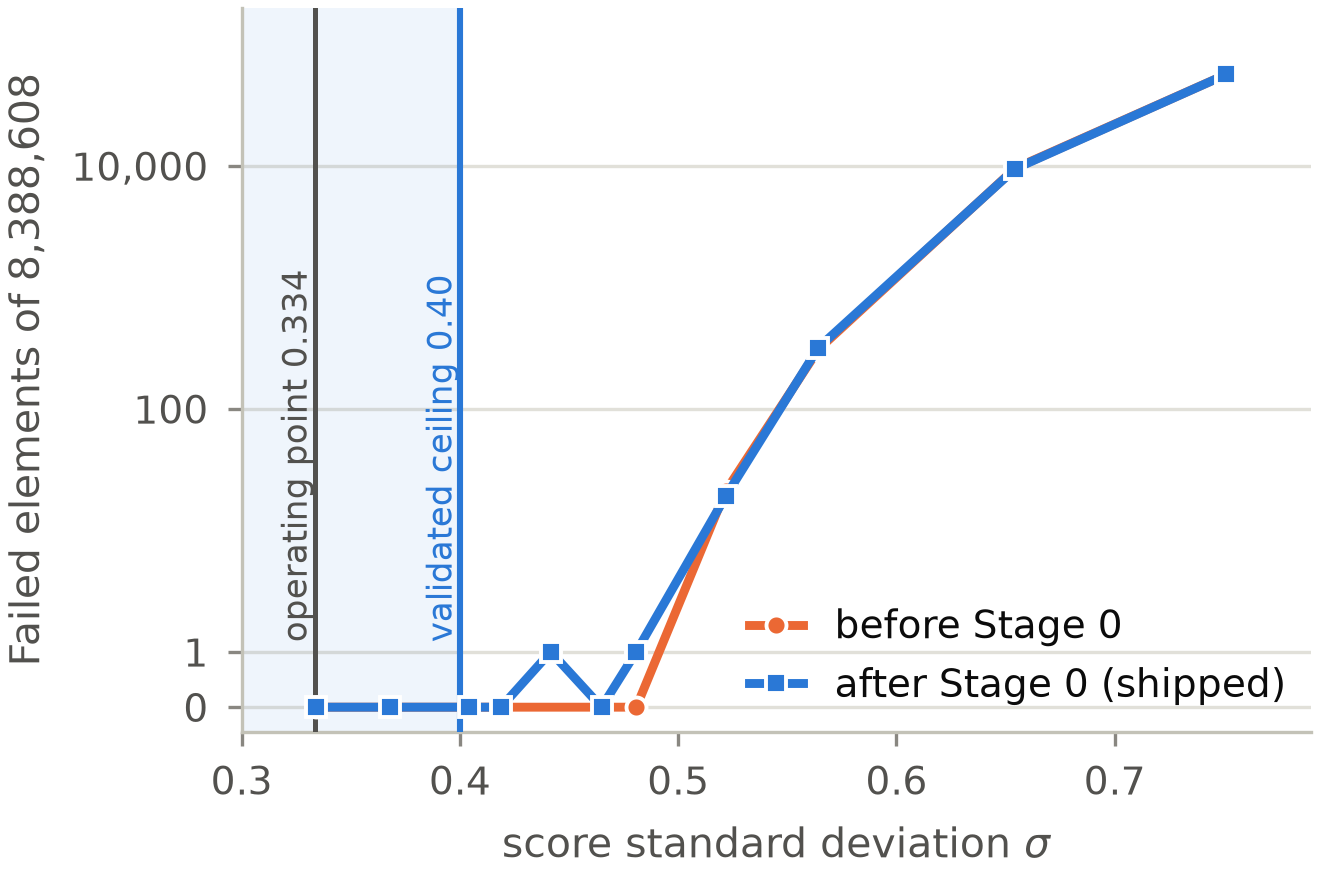
\includegraphics[width=\linewidth]{fig/sigma-guard-calibration.png}
\vspace{6pt}
\caption{Calibration of the polynomial route's runtime guard, at $N{=}8192$ against the dense reference. The shaded band is the admitted range.}
\label{fig:sigma}
\end{figure}

Finally, we believe that $\sigma$ is conservative for the target shape, because it was calibrated at $N{=}8192$ while attention contributes less to the residual stream as $N$ grows.

\section{Results}
\label{sec:results}

\subsection{Environment}
All results are obtained from the single machine in Table~\ref{tab:env}. The benchmark sets float32 matmul precision to \texttt{high}, enables TF32, uses input scale 1.0 with zero padding, and executes on CUDA 13.0.

\begin{table}[H]
\centering
\footnotesize
\begin{tabular}{p{2.1cm} p{5.4cm}}
\hline
\textbf{Component} & \textbf{Final benchmark machine} \\
\hline
CPU & AMD Ryzen 7 9800X3D, 8 cores / 16 threads \\
CPU cache & 384\,KiB L1d, 256\,KiB L1i, 8\,MiB L2, 96\,MiB L3 \\
GPU & NVIDIA GeForce RTX 5080, compute capability 12.0 \\
GPU memory & 16{,}303\,MiB \\
GPU limits & 360\,W; max queried SM clock 3{,}090\,MHz; memory clock 15{,}001\,MHz \\
Driver / CUDA & NVIDIA 616.56 / CUDA 13.0 \\
cuDNN & 9.2.0 \\
PyTorch / Triton & 2.13.0+cu130 / 3.7.1 \\
Python & 3.12.3 \\
OS & WSL2, Linux 6.6.114.1, x86-64, glibc 2.39 \\
Disk & 1{,}007\,GiB filesystem; 616\,GiB free before the run \\
\hline
\end{tabular}
\vspace{6pt}
\caption{Final benchmark environment.}
\label{tab:env}
\end{table}

Accuracy uses five seeds (1234--1238). Timing follows \S\ref{sec:timing}: paired interleaved CUDA events, 10\,s of settling per arm, 100 paired samples, and an automatically selected block targeting 50\,ms. Memory is probed after route compilation and replay are warm. The candidate is self-compiling and the harness refuses to wrap it in an external compiler.

\subsection{Cases 1--13}
Table~\ref{tab:results} and Figure~\ref{fig:speedup} give the directly comparable results. Every case passes 5/5 accuracy trials with zero failed elements, and every improvement clears its own noise floor. The geometric-mean speedup is \textbf{3.611$\times$}, ranging from 1.116$\times$ on projection-bound Case 8 to 8.577$\times$ on long-sequence Case 13.

\begin{table}[H]
\centering
\footnotesize
\begin{tabular}{r r r r r r}
\hline
\textbf{Case} & \textbf{Base ms} & \textbf{Cand.\ ms} & \textbf{Speedup} & \textbf{Noise} & \textbf{Max abs} \\
\hline
1  & 1.9350   & 0.6975  & 2.774$\times$ & 25.30\% & 0.001054 \\
2  & 1.1953   & 0.1609  & 7.428$\times$ & 62.49\% & 0.000819 \\
3  & 0.9788   & 0.1643  & 5.959$\times$ & 34.53\% & 0.000908 \\
4  & 1.1567   & 0.2678  & 4.319$\times$ & 17.64\% & 0.000908 \\
5  & 3.0159   & 1.2513  & 2.410$\times$ & 8.85\%  & 0.001181 \\
6  & 504.1028 & 210.5723& 2.394$\times$ & 0.52\%  & 0.001347 \\
7  & 1.5418   & 0.4060  & 3.797$\times$ & 33.12\% & 0.001316 \\
8  & 17.3913  & 15.5889 & 1.116$\times$ & 0.82\%  & 0.001218 \\
9  & 1.5037   & 0.6881  & 2.185$\times$ & 11.03\% & 0.001078 \\
10 & 1.8052   & 0.6464  & 2.793$\times$ & 20.44\% & 0.001089 \\
11 & 7.6778   & 1.3724  & 5.595$\times$ & 7.27\%  & 0.001063 \\
12 & 1.0901   & 0.2335  & 4.668$\times$ & 41.84\% & 0.001128 \\
13 & 116.7147 & 13.6078 & 8.577$\times$ & 9.12\%  & 0.001123 \\
\hline
\multicolumn{3}{l}{\textbf{Geometric mean}} & \textbf{3.611$\times$} & & \\
\hline
\end{tabular}
\vspace{6pt}
\caption{Final RTX 5080 results at commit \texttt{775c820}. Every row passes with zero failed elements, and significant speedup over noise per Eq.~\ref{eq:noise}.}
\label{tab:results}
\end{table}

\begin{figure}[H]
\centering
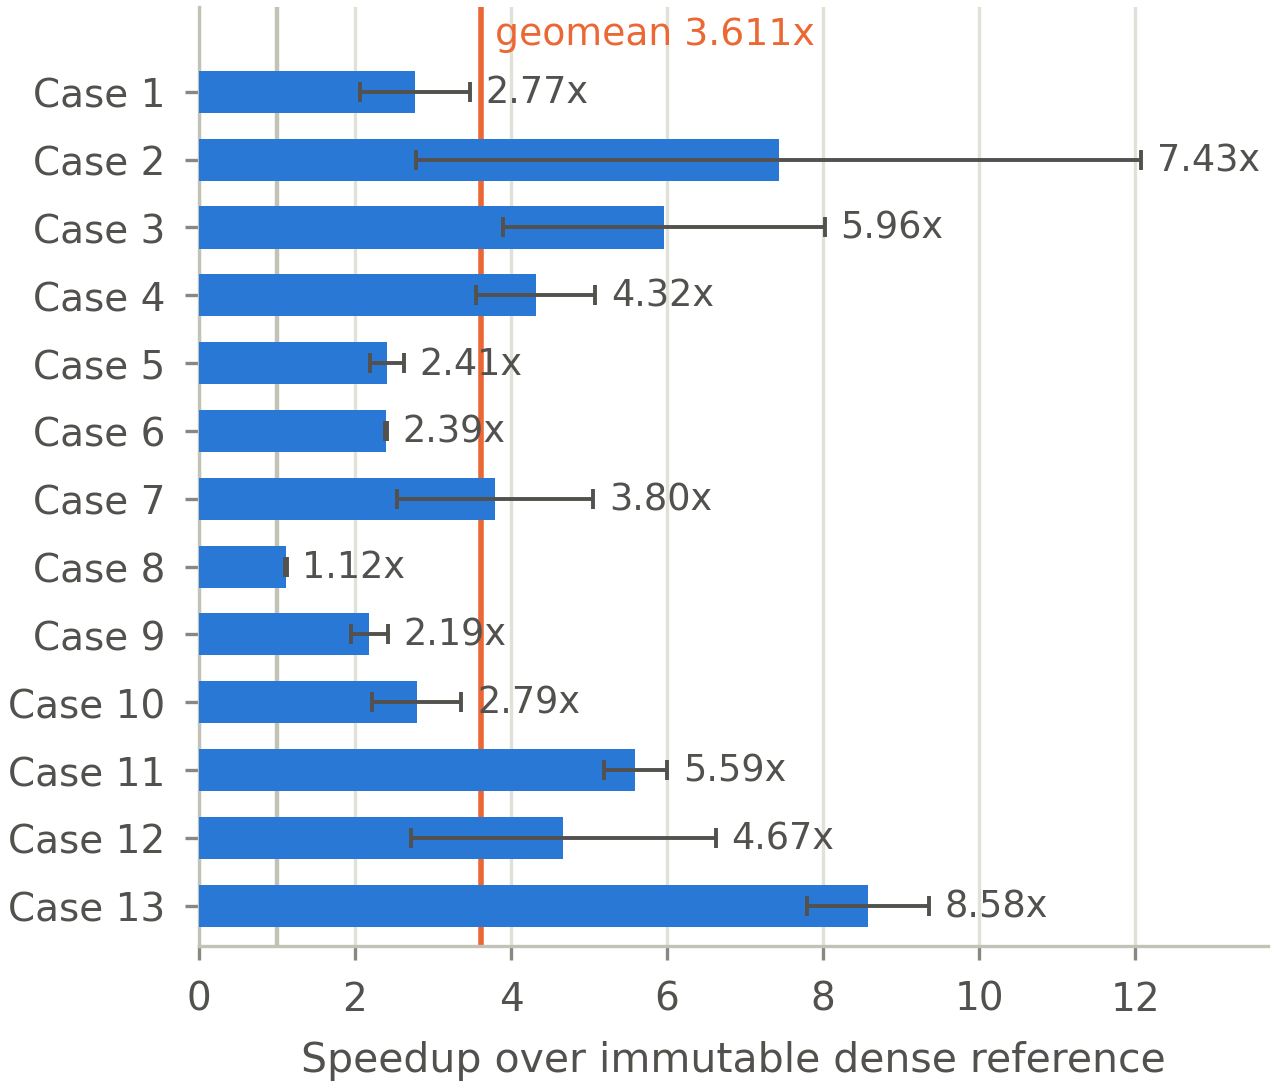
\includegraphics[width=\linewidth]{fig/speedup-by-case.png}
\vspace{6pt}
\caption{Per-case speedup over the immutable dense reference, with the run-specific 95\% noise floor of Eq.~\ref{eq:noise} as error bars. Wide bars belong to sub-millisecond shapes, where the measurement floor is wide.}
\label{fig:speedup}
\end{figure}

\begin{figure*}[t]
\centering
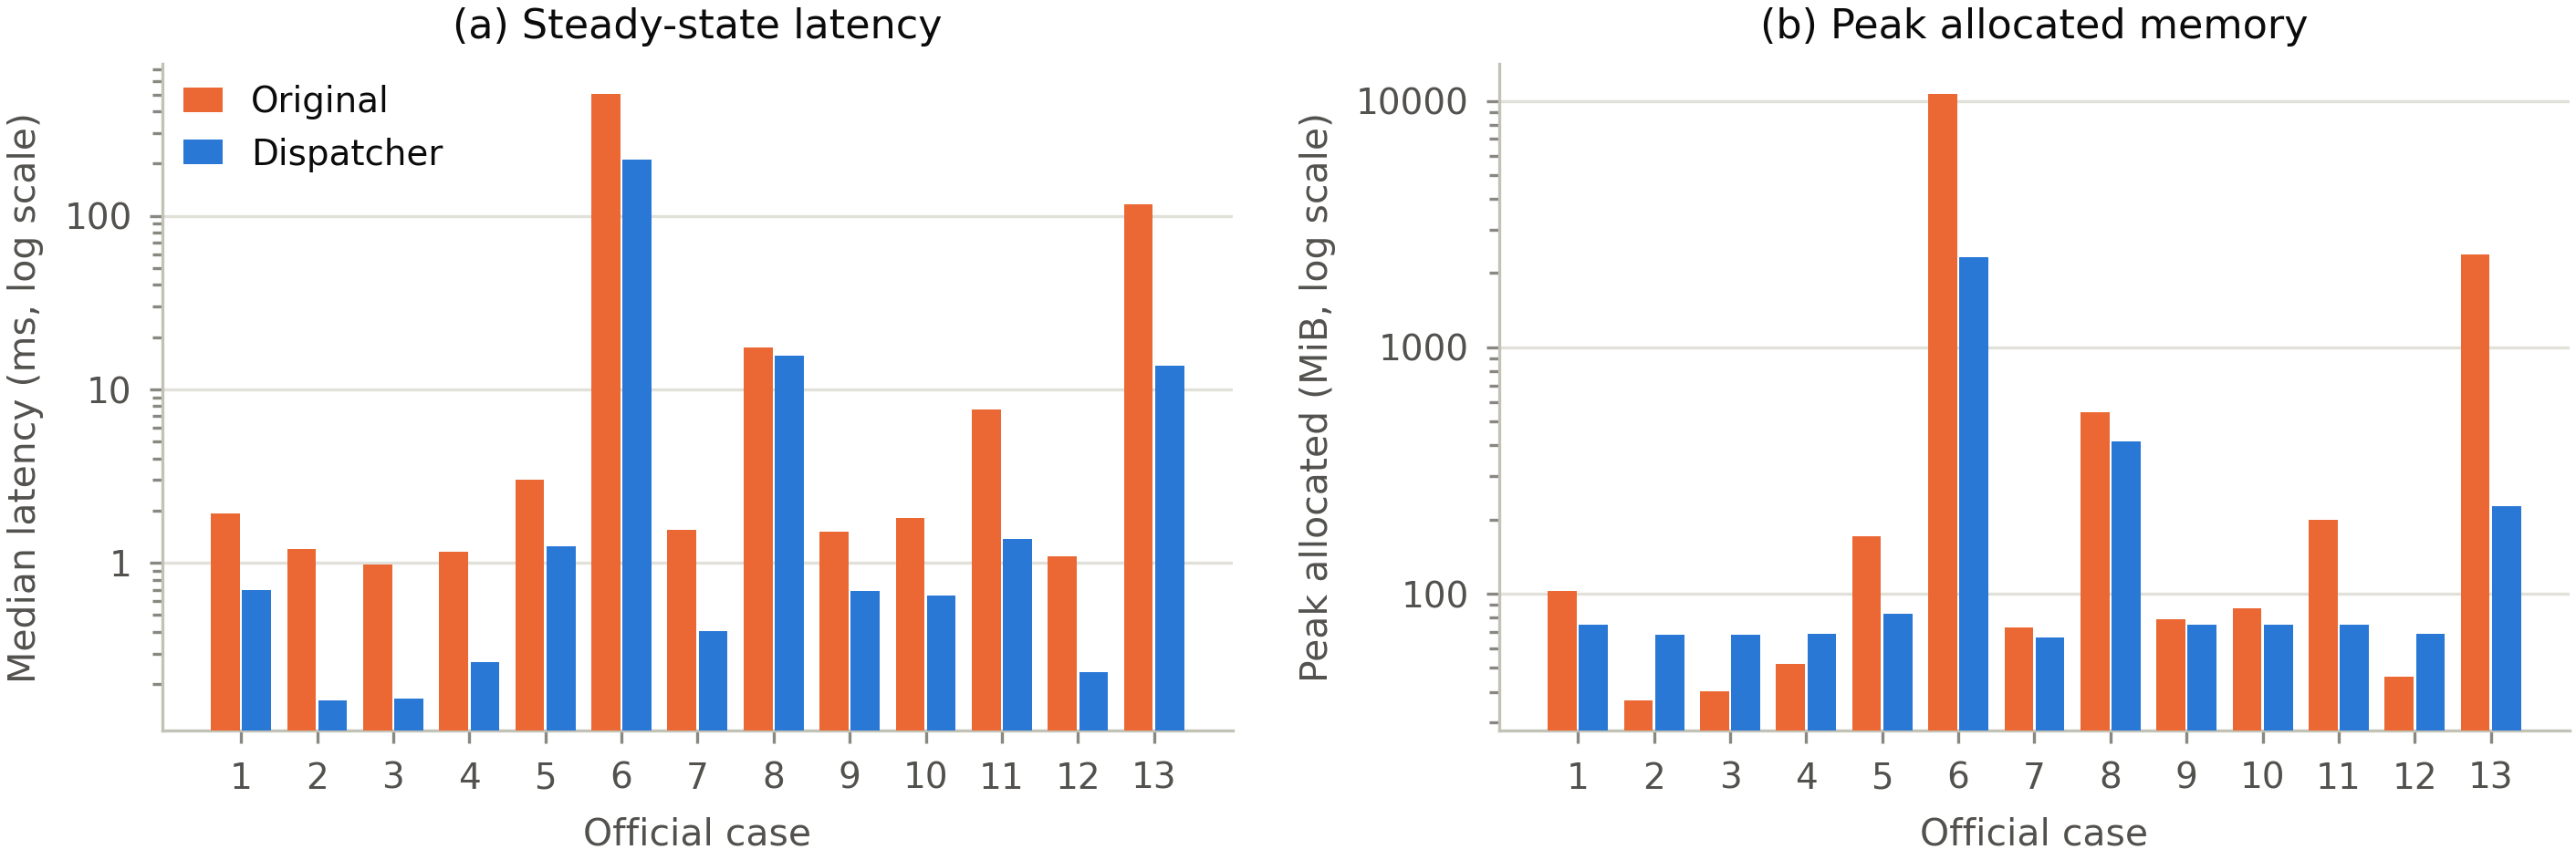
\includegraphics[width=\textwidth]{fig/latency-and-memory.png}
\vspace{6pt}
\caption{Cases 1--13 on the RTX 5080, both axes on log scales. (a) Median steady-state latency. (b) Peak allocated memory. The four cases where the candidate's peak is \emph{higher} --- 2, 3, 4 and 12 --- are all sub-millisecond shapes whose absolute peak is dominated by resident compiler caches rather than by model activations.}
\label{fig:latmem}
\end{figure*}

\subsection{Latency and Memory Together}
Figure~\ref{fig:latmem} plots both axes of the result, and the memory panel carries information the speedup table does not. On the two shapes where allocation is the binding constraint the reduction is decisive: Case 6 falls from 10{,}672.719\,MiB to 2{,}312.512\,MiB ($-78.3\%$) and Case 13 from 2{,}372.229\,MiB to 227.104\,MiB ($-90.4\%$).

The four cases where candidate peak allocation is higher than baseline are Cases 2, 3, 4 and 12, all under 70\,MiB in absolute terms. Those figures include resident Inductor and CUDA Graph caches and are not a standalone model-footprint measurement. We report them unadjusted rather than subtracting the compiler's own memory.

\subsection{Case 14}
Case 14 has no dense baseline, so it is reported separately and is \emph{not} folded into the 3.611$\times$ geometric mean. The immutable dense model cannot run at the target shape, and the reference accuracy checker independently exhausts memory at this output size because it retains full input, reference, and candidate tensors and then creates FP32 copies and boolean temporaries.

The harness therefore does four things. It validates a linear-memory FP32 oracle against the immutable dense model at $B{=}1$, $N{=}4096$, obtaining 0/4{,}194{,}304 failures at $\max_\text{abs}=0.00060248$. It generates one deterministic FP32 sample at a time at the full $B{=}32$, $N{=}100{,}000$, $d_\text{model}{=}1024$ shape. It passes that identical sample to both the oracle and the FP32-facing candidate. And it reduces the comparison in bounded token chunks, discarding each sample's outputs immediately. Table~\ref{tab:case14} gives the result.

\begin{table}[H]
\centering
\footnotesize
\begin{tabular}{p{2.6cm} p{4.9cm}}
\hline
\textbf{Quantity} & \textbf{Value} \\
\hline
Accuracy & PASS 5/5 trials, 0 failures across 16{,}384{,}000{,}000 elements \\
Max absolute error & 0.010294 (passes via the 2\% relative arm of Eq.~\ref{eq:tol}) \\
Mean absolute error & 0.000374 \\
Oracle time & 601.975\,s \\
Candidate time & 67.095\,s \\
Diagnostic ratio & 8.972$\times$ \\
Peak allocation & 3{,}643.988\,MiB \\
Measured $\sigma$ per layer & 0.3340, 0.3345 (guard ceiling 0.40) \\
\hline
\end{tabular}
\vspace{6pt}
\caption{Case 14 against the validated streamed FP32 oracle (a linear-memory proxy).}
\label{tab:case14}
\end{table}

\subsection{Regression Check}
The final implementation changes only Case 14 relative to branch base \texttt{3e6a3ea}. Cases 1--13 reproduce with no accuracy regression, and candidate latency moves between $-1.82\%$ and $+2.14\%$ --- within the noise floors of Table~\ref{tab:results} on every row. The CUDA-aware unit suite (210 tests, including dispatcher and kernel coverage) passes.

\section{Discussion}

\subsection{Performance optimizations}
The speedup pattern follows the regime classification of Table~\ref{tab:shapes} almost exactly. The largest gains are on memory-bound attention (Case 13 at 8.577$\times$, Case 11 at 5.595$\times$), where removing the score tensor from memory removes most of the runtime. The next largest are on launch-bound shapes (Case 2 at 7.428$\times$), where CUDA Graph replay removes per-call dispatch that was most of the measured time. The smallest is on projection-bound Case 8 at 1.116$\times$, and this is a ceiling rather than a shortfall: attention is only 15.7\% of that shape's work, so even perfect attention leaves the dense GEMMs untouched. We probed those GEMMs directly, expanding 727 valid cuBLASLt algorithm configurations per layout, and the best admissible bias-plus-residual epilogue projected only about 1.010$\times$ whole-model. That route was rejected before integration.

\subsection{Large Noise Floors}
Seven of the thirteen cases have noise floors above 17\%. It would be easy to present tighter numbers by timing a single arm after a long warmup, and it would be wrong. These are shapes whose entire forward pass takes between 0.16\,ms and 1.9\,ms depending on the arm, on a GPU whose clocks move by a factor of two; a 20\% measurement floor is what that machine can actually resolve, and Eq.~\ref{eq:noise} reports it rather than hiding it. The corresponding gains on those seven rows are 2.8--7.4$\times$, so the conclusions are unaffected, but the exact point estimates on those rows may move between runs and should not be over-read.

\subsection{Generality}
The polynomial route is the one component that is benchmark-specific by construction, and we would rather say so plainly than let the runtime guard imply otherwise. It works because $\sigma \approx 0.334$ is a consequence of the benchmark's default \texttt{nn.Linear} initialization: a LayerNormed input gives $q,k$ component RMS 0.577, which fixes the score spread independently of $N$ and of $d_\text{model}$. Under trained weights the softmax is peaked and a degree-2 fit would be poor. Everything else in the dispatcher --- SDPA substitution, strided views, mask elimination, packed QKV, batch and prefix streaming --- is a standard optimization that transfers.

\section{Rejected Optimizations}
\label{sec:negative}
Table~\ref{tab:negative} lists directions that were implemented or measured and then rejected. Each cost real measurement time, and each closes a plausible-looking path.

\begin{table}[H]
\centering
\scriptsize
\begin{tabular}{p{2.35cm} p{2.2cm} p{2.6cm}}
\hline
\textbf{Direction} & \textbf{Measured} & \textbf{Why rejected} \\
\hline
\texttt{max-autotune} everywhere & Case 8 FAIL 5/5, 7{,}899 bad elements & No runtime gain over \texttt{reduce-overhead} and it breaks the criterion \\
Whole-model FP16 & Cases 7, 13 FAIL & Reference rounds probabilities to fp16 before $PV$; even folding \texttt{scale} breaks it \\
FP16 attention internals (fp32 cases) & PASS, but slower & Cast overhead exceeds the tensor-core throughput at these sizes \\
Universal packed QKV & Case 8 1.003$\times$ & Below the noise floor; kept only for Cases 2 and 3 \\
Selective GEMM autotuning, prepacked weights & Neutral & No measurable gain, and autotuning was numerically invalid \\
Direct cuBLASLt Case-8 epilogue & 727 configs; 1.010$\times$ projected & Amdahl ceiling too low to justify integration \\
Triton output/residual fusion (Case 5) & $\approx$9\% faster & 22{,}132 stress-matrix elements fail \\
Order-1 linear attention (Case 14) & 4.36$\times$ & 957 failures at $N{=}65536$; the quadratic term is required \\
fp16 polynomial state & 1.32$\times$ & Passes at $N{=}16384$, fails at $N{=}65536$ with 1{,}064{,}935 failures \\
Symmetric feature packing & 750.5 vs 526.7\,ms & The two gathers cost more than the bandwidth saved \\
Sparse / top-$k$ attention (Case 14) & 89\% effective softmax support & Nothing to prune: top-64 keys hold 3.4\% of the mass \\
Persistent-slab scan (Case 14) & Kernels at 24--27 TFLOPS & No longer traffic-limited after Stage 0; the premise expired \\
\hline
\end{tabular}
\vspace{6pt}
\caption{Measured and rejected directions.}
\label{tab:negative}
\end{table}

Two entries deserve emphasis. The fp16 polynomial state is a trap: it is the fastest correct-\emph{looking} option and passes every cheap small-$N$ test, failing only at the scale that matters, because several hundred chunk contributions accumulate and small increments are lost against a large fp16 accumulator. And the sparse-attention exclusion is worth more than the argument it replaced --- the original reasoning was that any approximation must fail a per-element tolerance, which is false as stated; the measurement that the softmax over 100{,}000 keys has 89\% effective support is both true and independent of the tolerance.

\section*{Reproduction}
The repository is at \url{https://github.com/IceyFoxes/techjam}. Figures in this report are regenerated from the preserved benchmark JSON by \texttt{docs/make\_figures.py}. Any directly comparable case runs as shown in Listing~\ref{lst:repro}, substituting \texttt{-{}-case} 1 through 13.

\begin{lstlisting}[style=code,caption={Reproducing one official case.},label={lst:repro}]
.venv/bin/python -m src.benchmark \
  --candidate src.dispatcher --case 6 \
  --device cuda --dtype float32 \
  --accuracy-trials 5 --seed 1234 \
  --warmup 20 --repeats 100 --benchmark-rounds 3 \
  --timing paired --settle-seconds 10 \
  --output research/benchmarks/DATE-GPU-COMMIT/result.json
\end{lstlisting}

\newpage
\begin{thebibliography}{1}

\bibitem{flash2}
T.~Dao, ``FlashAttention-2: Faster attention with better parallelism and work partitioning,'' in \emph{Proc. Int. Conf. Learning Representations (ICLR)}, 2024. [Online]. Available: \url{https://arxiv.org/abs/2307.08691}

\bibitem{rabe}
M.~N. Rabe and C.~Staats, ``Self-attention does not need $O(n^2)$ memory,'' arXiv:2112.05682, 2021.

\bibitem{online}
M.~Milakov and N.~Gimelshein, ``Online normalizer calculation for softmax,'' arXiv:1805.02867, 2018.

\bibitem{based}
S.~Arora, S.~Eyuboglu, M.~Zhang, et al., ``Simple linear attention language models balance the recall-throughput tradeoff,'' in \emph{Proc. Int. Conf. Machine Learning (ICML)}, 2024. [Online]. Available: \url{https://arxiv.org/abs/2402.18668}

\bibitem{katharopoulos}
A.~Katharopoulos, A.~Vyas, N.~Pappas, and F.~Fleuret, ``Transformers are RNNs: Fast autoregressive transformers with linear attention,'' in \emph{Proc. Int. Conf. Machine Learning (ICML)}, 2020.

\bibitem{performer}
K.~Choromanski, V.~Likhosherstov, D.~Dohan, et al., ``Rethinking attention with Performers,'' in \emph{Proc. Int. Conf. Learning Representations (ICLR)}, 2021.

\bibitem{quest}
J.~Tang, Y.~Zhao, K.~Zhu, G.~Xiao, B.~Kasikci, and S.~Han, ``Quest: Query-aware sparsity for efficient long-context LLM inference,'' in \emph{Proc. Int. Conf. Machine Learning (ICML)}, 2024.

\bibitem{minference}
H.~Jiang, Y.~Li, C.~Zhang, et al., ``MInference 1.0: Accelerating pre-filling for long-context LLMs via dynamic sparse attention,'' in \emph{Advances in Neural Information Processing Systems (NeurIPS)}, 2024.

\bibitem{triton}
P.~Tillet, H.~T. Kung, and D.~Cox, ``Triton: An intermediate language and compiler for tiled neural network computations,'' in \emph{Proc. 3rd ACM SIGPLAN Int. Workshop on Machine Learning and Programming Languages (MAPL)}, 2019, pp. 10--19.

\bibitem{pt2}
J.~Ansel, E.~Yang, H.~He, et al., ``PyTorch 2: Faster machine learning through dynamic Python bytecode transformation and graph compilation,'' in \emph{Proc. 29th ACM Int. Conf. Architectural Support for Programming Languages and Operating Systems (ASPLOS)}, 2024.

\bibitem{sdpa}
PyTorch, ``torch.nn.functional.scaled\_dot\_product\_attention,'' PyTorch documentation. Accessed 29 August 2026. [Online]. Available: \url{https://docs.pytorch.org/docs/main/generated/torch.nn.functional.scaled_dot_product_attention.html}

\end{thebibliography}

\end{document}
